\chapter{Standard Model Muon decay}
\label{ch:SMMuon}
The muon exhibits only three standard model decay modes, namely $\mu^-\rightarrow e^-\bar{\nu}_e\nu_\mu$, the corresponding radiative mode $\mu^-\rightarrow e^-\bar{\nu}_e\nu_\mu\gamma$ and $\mu^-\rightarrow e^-\bar{\nu}_e\nu_\mu e^+e^-$. The former is seen in almost every muon decay, while the last two combined are responsible for less than one in every 10.000 decays so its justified to assume the muon has only one decay mode. This clean background and the straightforward production and detection render the muon decay a great proving ground for the weak interaction. This can be turned around to set Fermis coupling constant by matching it to the muon lifetime.
Even though being investigated there is no sign of other decay modes beyond the standard model that would point to new physics. 
\begin{figure}[H]
\centering
\begin{tikzpicture}
\begin{feynman}
\vertex (a) {\(\mu^{-}\)};
\vertex [right=of a] (b);
\vertex [above right=of b] (f1){\(\nu_\mu \)};
\vertex [below right=of b] (c);
\vertex [above right=of c] (f2){\(e^-\)};
\vertex [below right=of c] (f3){\(\bar{\nu}_e\)};
\diagram* {
(a)--[fermion](b)--[fermion](f1),
(b)--[boson, edge label'=\(W\)](c),
(f2)--[anti fermion](c)--[anti fermion](f3)};
\end{feynman}
\end{tikzpicture}
\caption{Standard model muon decay mediated by the V-A interaction}
\label{fg:SM-Muondecay}
\end{figure}
The decay is mediated by the charged current interaction as shown in diagram \ref{fg:SM-Muondecay}. New physics might alter the V-A structure such that the angular distribution of the electrons momentum relative to the polarisation of the muon is sensitive to deviations from the standard model.  

To this end its important to understand the standard model induced structure of the decay. Assigning momenta $P,P_{\nu_\mu},P_e,P_{\nu_e}$ and polarisations $s,s_{\nu_\mu},s_e,s_{\nu_e}$ to the $\mu^-,\nu_\mu,e^-$ and $\bar{\nu}_e$ respectively
 and neglecting the momentum transfer in the W-propagator the corresponding matrix element is
 \begin{equation}
 -i\mathcal{M}=\frac{-ig^2}{8m_W^2}\bar{u}(P_{\nu_\mu},s_{\nu_\mu}) \gamma_\mu(1-\gamma^5)u(P,s)\bar{u}(P_e,s_e)\gamma^\mu(1-\gamma^5)v(P_{\nu_e},s_{\nu_e}).
 \end{equation}
In the squared matrix element there will be a term proportional to $u(P,s)\bar{u}(P,s)$ that is replaced by 
\begin{equation}
u(P,s)\bar{u}(P,s)=(\slashed{P}+m_\mu)\frac{1+\gamma^5\slashed{S}}{2}
\end{equation}
where $\slashed{S}$ contains the spin four-vector of the muon.
Summing over the final state polarisations since its not measured this results in
\begin{equation}
|\mathcal{M}|^2=\frac{2g^4}{M_w^4} (P_{\nu_\mu} \cdot P_e ) (P-m_\mu S)\cdot P_{\nu_e}.
\end{equation}
All that is left is the phase space integration
\begin{equation}
d\Gamma = \frac{1}{2m_\mu}\frac{1}{2E_e}\frac{d^3p_e}{(2\pi)^2}\frac{1}{2E_{\nu_e}}\frac{d^3p_{\nu_e}}{(2\pi)^2}\frac{1}{2E_{\nu_\mu}}\frac{d^3p_{\nu_\mu}}{(2\pi)^2}|\mathcal{M}|^2(2\pi)^4\delta^{(4)}(P-P_e-P_{\nu_\mu}-P_{\nu_e})
\end{equation}
 while leaving out the integral over the electrons energy and the angle $\theta$ between the electron momentum and the muon spin to get the decay spectrum. 
This is written with the new variable $x=2E_e/m_\mu$ as the electron energy normalised to the maximum value and the Fermi coupling $G_f=g^2/(4\sqrt{2}m_W^2)$ as
\begin{align}
\frac{d^2\Gamma}{dxd\cos\theta}=\frac{G_f^2m_\mu^5}{192\pi^3}\left[x^2\left((3-2x)+(1-2x)\cos\theta\right)\right]
\label{eq:DiffrateSimple}
\end{align}
where the term outside the square brackets is the total decay width.
\begin{figure}[H]
  \centering
    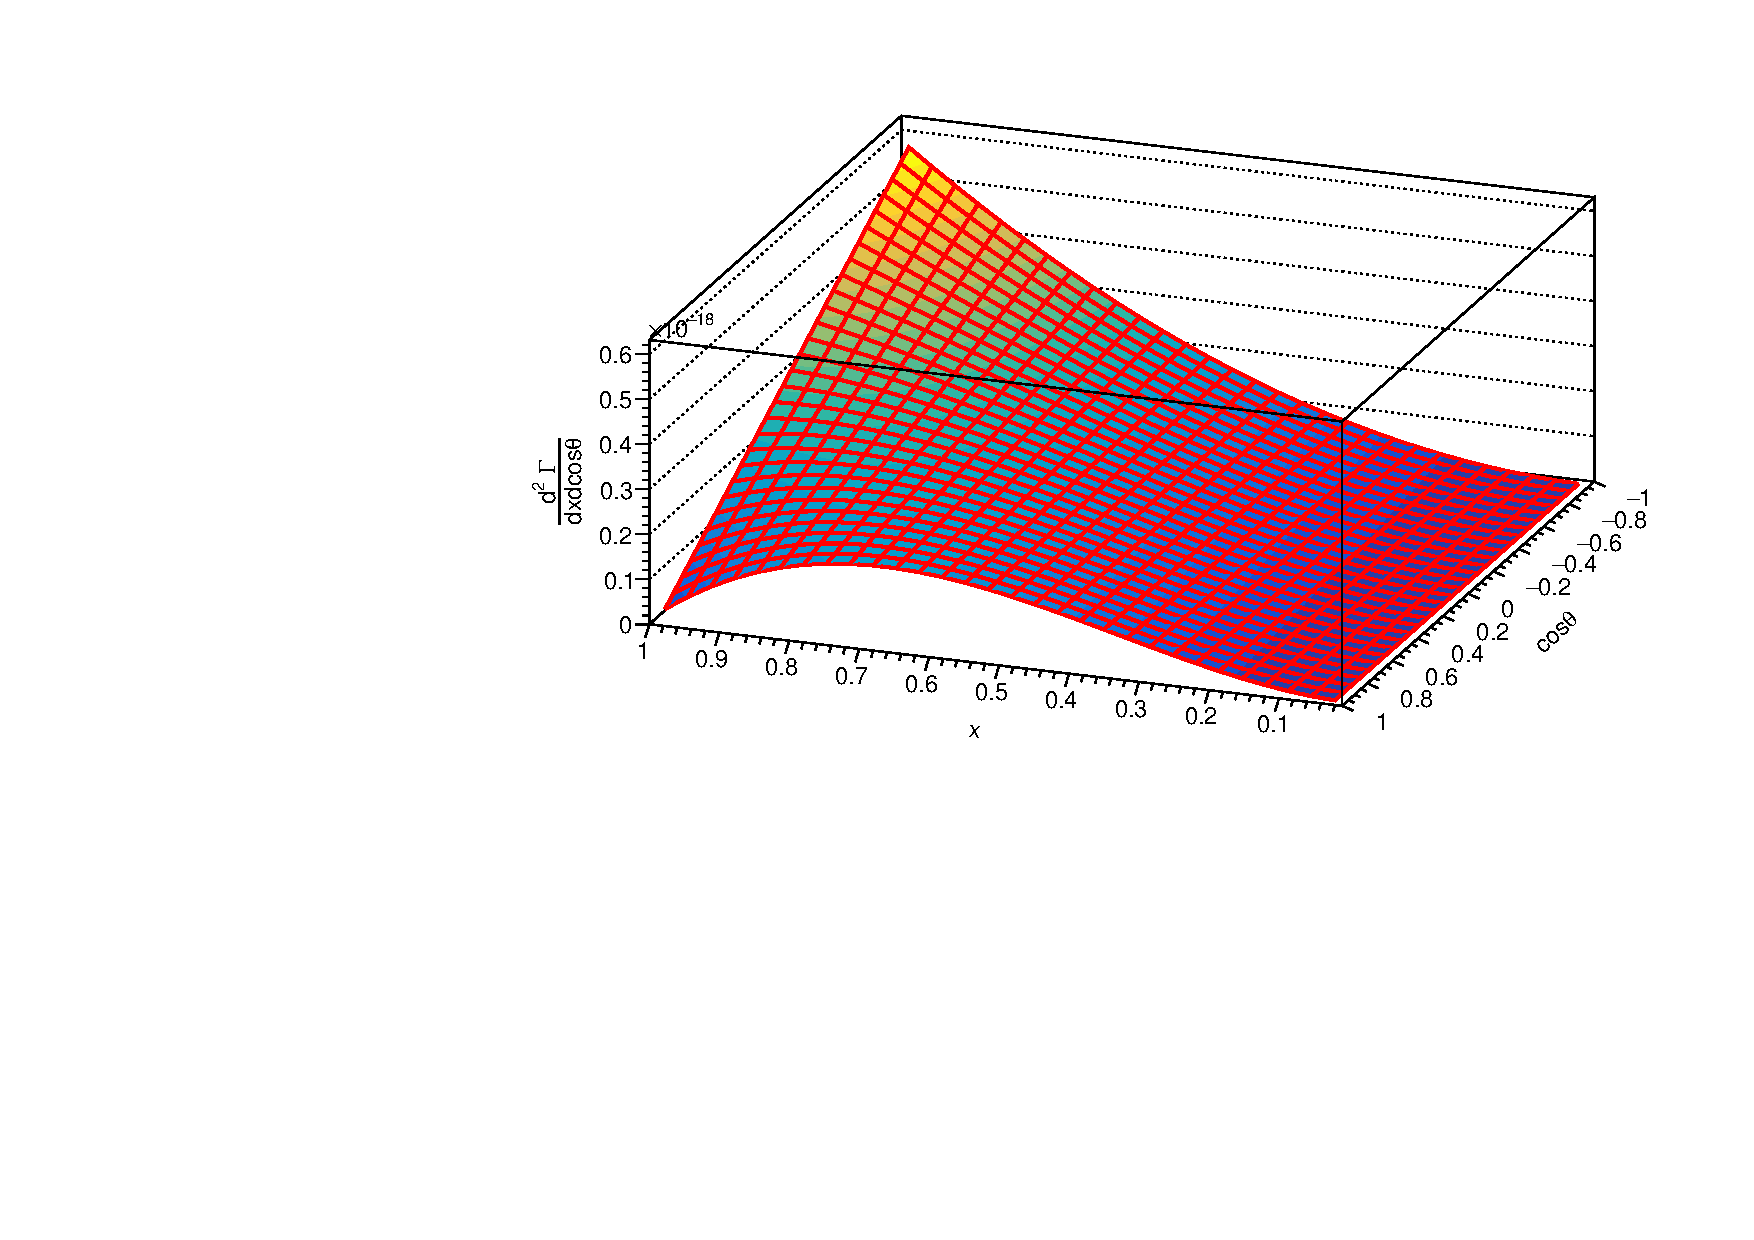
\includegraphics[width=0.8\textwidth]{imgs/MuonSpectrum}
    \caption{Standard model muon decay spectrum}
    \label{fg:SM-MuonSpectrum}
\end{figure}
The corresponding spectrum is shown in figure \ref{fg:SM-MuonSpectrum}.
If one were not to neglect the electron mass the calculation gets a bit more messy, but leads to the more precise result
\begin{equation}
\frac{d^2\Gamma}{dxd\cos\theta}=\frac{m_\mu}{4\pi^3} W_{e\mu}^4G_f^2\sqrt{x^2-x_0^2}\left(F_{\text{IS}}(x)-P_\mu\cos\theta F_{\text{AS}}(x)\right)
\label{eq:Diffrate}
\end{equation}
 with $W_{e\mu}$ as the maximum electron energy $(m_\mu^2+m_e^2)/2m_\mu$, $x_0$ the minimum electron energy $m_e/W_{e\mu}$, $P_\mu$ the degree of muon polarisation and the functions for the isotropic part $F_\text{IS}(x)$ and the anisotropic part $F_\text{AS}(x)$ given below \cite{Patrignani:2016xqp}.
\begin{align*}
F_\text{IS}&=x(1-x)+\frac{2}{9}\rho(4x^2-3x-x_0^2)+\eta x_0(1-x)\\
F_\text{AS}&=\frac{1}{3}\xi\sqrt{x^2-x_0^2}\left[1-x+\frac{2}{3}\delta(4x-4+\sqrt{1-x_0^2}\right]
\end{align*} 
Here the Michel parameters $\rho,\eta,\xi$ and $\delta$ have been introduced. The corresponding standard model values can be found by comparison of coefficients between equation \ref{eq:DiffrateSimple} and \ref{eq:Diffrate} and are $3/4$, $0$, $1$ and  $3/4$ respectively.
These can also be used to parametrise additional contributions to the muon decay that can be expressed as an effective four point interaction. These matrix elements can then be written as \cite{Patrignani:2016xqp}:
\begin{equation}
\frac{4G_f}{\sqrt{2}}\sum_{\substack{\gamma=\text{S,V,T}\\\epsilon,\mu = \text{R,L}}}g_{\epsilon\mu}^\gamma \langle\bar{e}_\epsilon \lvert \Gamma^\gamma \lvert (\nu_e)_n \rangle\langle (\bar{\nu}_\mu)_m \lvert \Gamma_\gamma \lvert \mu_\mu \rangle
\end{equation}
where the indices S,V,T denote scalar, vector and tensor interactions respectively while $\Gamma$ represents the corresponding operators and the R/L indices indicate the chirality of the fermions.
The amplitudes $g_{\epsilon\mu}^\gamma$ can then be combined to 
\begin{align*}
a&= 16( \lvert g_\text{RL}^V \lvert ^2 + \lvert g_\text{LR}^V \lvert ^2)+ \lvert g_\text{RL}^S + 6g_\text{RL}^T \lvert ^2+ \lvert g_\text{LR}^S + 6g_\text{LR}^T \lvert ^2  \\
a'&=16( \lvert g_\text{RL}^V \lvert ^2 - \lvert g_\text{LR}^V \lvert ^2)+ \lvert g_\text{RL}^S + 6g_\text{RL}^T \lvert ^2- \lvert g_\text{LR}^S + 6g_\text{LR}^T \lvert ^2 \\
b&=4(\lvert g_\text{RR}^V \lvert^2+\lvert g_\text{LL}^V \lvert ^2)+\lvert g_\text{RR}^S \lvert ^2+\lvert g_\text{LL}^S \lvert ^2\\
b'&=4(\lvert g_\text{RR}^V \lvert^2-\lvert g_\text{LL}^V \lvert ^2)+\lvert g_\text{RR}^S \lvert ^2-\lvert g_\text{LL}^S \lvert ^2\\
c&=\frac{1}{2}(\lvert g_\text{RL}^S -2g_\text{RL}^T \lvert ^2+\lvert g_\text{LR}^S -2g_\text{LR}^T \lvert ^2)\\
c'&=\frac{1}{2}(\lvert g_\text{RL}^S -2g_\text{RL}^T \lvert ^2-\lvert g_\text{LR}^S -2g_\text{LR}^T \lvert ^2)\\
\alpha &= 8\Re (g_\text{RL}^V(g_\text{LR}^{S*}+6g_\text{LR}^{T*})+g_\text{LR}^V(g_\text{RL}^{S*}+6g_\text{RL}^{T*}))\\
\beta &=-4\Re (g_\text{RR}^V g_\text{LL}^{S*}+g_\text{LL}^V g_\text{RR}^{S*})
\end{align*}
which is a parametrisation that has also been experimentally measured. In terms of these the Michel parameters are given by:
\begin{align}
\rho -\frac{3}{4}&= \frac{3}{4}\frac{2c -a }{a+4b+6c}\\
\eta &=\frac{\alpha -2\beta}{a+4b+6c}\\
\delta -\frac{3}{4}&=\frac{9}{4}\frac{2c'-a'}{3a'+4b'-14c'}\\
1-\xi\frac{\delta}{\rho}&=\frac{b+b'+2(c-c')}{b+2c}
\end{align}
The standard model alone leads to all amplitudes to vanish except $g_{LL}^V =1$.
 
\paragraph{Experimental test}
The most recent and precise measurement of the Michel parameters $\rho$, $\delta$ and $P_\mu\xi$ has been done by the TWIST Collaboration \cite{TWIST:2011aa}. The experiment used the proton beam at TRIUMF accelerator in Vancouver. The protons were dumped on a carbon target, creating pions of which some decay in the material via the two body decay shown in chapter \ref{ch:SM-PionDecay}. These at the time 100\% polarised muons are then stopped at a silver or aluminium foil-target in the TWIST detector. In the time between the creation and decay the muons depolarise. This has to be corrected in the analysis. Then the momentum-angle distribution of the resulting positrons was measured. The analysis was done blind. Decay parameters were chosen randomly close to the expected values before the analysis and the corresponding Monte Carlo spectrum $S_\text{MC}$ including radiative corrections with a detector simulation was generated while the chosen parameters are kept hidden to avoid any human bias. The analysis is then done to extract $\Delta\rho$, $\Delta (P_\mu \xi)$ and $\Delta( P_\mu\xi\delta)$ from
\begin{equation}
S_\text{Data}=S_\text{MC}+\frac{\partial S}{\partial\rho}\Delta \rho+\frac{\partial S}{\partial P_\mu\xi}\Delta(P_\mu\xi)+\frac{\partial S}{\partial P_\mu \xi \delta}\Delta(P_\mu\xi\delta)
\end{equation}
After these parameters were extracted and the uncertainties were determined the hidden parameters can be revealed and the full result calculated. 
The results are :
\begin{align*}
\rho &= 0.74977\pm0.00012(\text{stat.})\pm 0.00023(\text{sys.})\\
\delta &=0.75049\pm0.00021(\text{stat.})\pm 0.00027(\text{syst.})\\
P^\pi_\mu\xi\delta/\rho&=1.00170^{+0.00156}_{-0.00071}
\end{align*}

Including these results, a global analysis results in 
\begin{align*}
\rho &=0.74979 \pm 0.00026\\
\eta &=0.057 \pm 0.034\\
\delta &= 0.75047\pm 0.00034\\
\xi &= 1.0009^{+0.0016}_{-0.0007}
\end{align*}
and is used for the following constraining of the dark matter mediators.